\documentclass[sigconf,nonacm]{acmart}

\settopmatter{printacmref=false}
\renewcommand\footnotetextcopyrightpermission[1]{}
\pagestyle{plain}

\usepackage{booktabs}
\usepackage{graphicx}
\usepackage{subcaption}
\usepackage{tabularx}
\usepackage{array}
\usepackage{amsmath,amssymb}
\usepackage{microtype}

% ---- BEGIN-CUSTOM (layout helpers; no content) ----
% Allow line breaks after underscores (file names, slice IDs, config keys)
% so long \texttt{...}/\textsf{...} identifiers never run into the margin.
\makeatletter
\DeclareRobustCommand{\_}{\ifmmode\nfss@text{\textunderscore}\else\textunderscore\allowbreak\fi}
\makeatother
% Breakable protocol file name
\newcommand{\protocolfile}{\texttt{configs/\allowbreak protocol.yaml}}
% Left-aligned, wrapping column for tabularx
\newcolumntype{Y}{>{\raggedright\arraybackslash}X}
% Keep floats and lists tidy
\setlength{\emergencystretch}{2em}
% Scale a wide table down ONLY if it is wider than the given width
\newsavebox{\fitbox}
\newcommand{\fitwidth}[2]{%
  \sbox{\fitbox}{#2}%
  \ifdim\wd\fitbox>#1\relax
    \resizebox{#1}{!}{\usebox{\fitbox}}%
  \else
    \usebox{\fitbox}%
  \fi}
% Let large floats sit close to where they are first mentioned
\renewcommand{\topfraction}{0.9}
\renewcommand{\dbltopfraction}{0.9}
\renewcommand{\textfraction}{0.1}
\renewcommand{\floatpagefraction}{0.7}
\renewcommand{\dblfloatpagefraction}{0.7}
\setcounter{topnumber}{3}
\setcounter{dbltopnumber}{4}
\setcounter{totalnumber}{6}
% ---- END-CUSTOM ----

\title{Are Factuality Scores Interchangeable? A Controlled Multi-Metric Evaluation of Small Open Large Language Models on Scientific Question Answering}

\author{Aman Kumar Emaley}
\affiliation{%
  \institution{Indian Institute of Information Technology, Allahabad}
  \department{Department of Information Technology}
  \city{Prayagraj}
  \state{Uttar Pradesh}
  \country{India}
}
\email{mcl2026012@iiita.ac.in}

\begin{document}

\begin{abstract}
The most frequently used scalar metric for assesssing large language models (LLMs) on scientific tasks is top-1 raw accuracy. We use an empirical approach to determine if factuality metrics agree on model rankings for five scientific slices across biomedicine, mathematics, and physical sciences (950 unique items, 1,450 evaluations per item slice). We apply three open-weights instruction-tuned models: \textsf{Qwen2.5-1.5B-Instruct}, \textsf{Qwen2.5-7B-Instruct} (using 4-bit quantization; evaluation performed using the same protocol as 4-bit Qwen2.5-7B-Instruct) and \textsf{Phi-3.5-mini-instruct} to a fixed protocol (\textbf{FactBench}) to test accuracy, multiclass Brier score (Bias-in-between labels, [0, 2]), Expected Calibration Error (ECE), selective prediction risk (AURC), confidence discrimination ($\text{AUROC}_{\text{conf}}$), and permutation consistency, followed by execution of 17,400 forward passes across 17,000 models and 3,000 prompts each. The main findings from our empirical results are the following: (1) \textbf{Metric Discordance:} Model rankings using probability calibration (ECE) and confidence discrimination ($\text{AUROC}_{\text{conf}}$) differ from raw accuracy rankings, and Brier score, AURC, and selective accuracy are strongly correlated (mean within-slice Kendall $\tau \approx 0.830$). On biomedical MMLU, \textsf{Phi-3.5-mini} obtains the highest raw accuracy (77.3\%), and lowest confidence discrimination ($\text{AUROC}_{\text{conf}} = 0.703$), with statistically not significant differences over the three biomedical pairs (Holm-adjusted paired $p$ values range from 0.35 to 0.98), suggesting that rank differences are suggestive when $N=3$ models. We find that models persistently predict an answer that is clearly wrong, even if very confidently, not being detected by permutation consistency: (0.2) \textbf{The Consistency Trap}: There are 1,029 item-model error instances, in which the model predicts the same erroneous response for all four possible response orderings with high mean confidence (0.949 on average across all cells, up to 1.000 for \textbf{Phi-3.5} on biomed); the 55.2\% majority repeat the same inaccurate response by chance at best, evidences a strong ``yes'' bias, and results in a Brier score drop of more than 0.57 with context in the PubMedQA setting (paired exact McNemar $p < 0.001$). We believe there is a need for multidimensional reporting vectors, with accuracy, calibration, abstention, and evidence grounding separated from each other in the case of scientific LLM benchmarking.
\end{abstract}

\begin{CCSXML}
<ccs2012>
   <concept>
       <concept_id>10010147.10010178.10010179</concept_id>
       <concept_desc>Computing methodologies~Natural language processing</concept_desc>
       <concept_significance>500</concept_significance>
   </concept>
</ccs2012>
\end{CCSXML}

\keywords{Large Language Models (LLM) and Scientific Question Answering, Factuality Metric, Calibration and Selective Prediction, Permutation Consistency}

\maketitle

\section{Introduction}
Large language models (LLMs) are increasingly being utilized in diverse aspects of scientific research, including biomedical literature summarization, medical research filtering, and solving physics and chemistry problems~\cite{hendrycks2021mmlu,jin2019pubmedqa}. Typically, to assess an LLM's ability to perform in science, it is tested on multiple choice question (MCQ) answering benchmarks, where one scalar number (top-1 raw accuracy) is published on public leaderboards. In areas of science where a wrong claim could cause incorrect lab experiments or medical or therapeutic advice, however, an agreeable conversational style or a very high accuracy score tells little of whether the model's confidence is correlated with truth or whether it can safely withhold its answer under epistemic uncertainty, or whether its answers fall apart when the immediate retrieved evidence is removed~\cite{guo2017calibration,geifman2017selective,kadavath2022language}.

As a category, factuality in science has structural dimensions, not just one monolithic dimension. A scientific model could accurately quote a biological terminology definition, but incorrectly describe the clinical context of a therapy, solve a quantitative physics problem with an incorrect physical assumption, reference a real paper that is relevant but that the modeler is certain does not support the claim, and assert a multiple choice answer without acknowledging that the study results that support it are ambiguous. Therefore, there is no single top-1 accuracy score that will give confidence in the reliability or safety of an AI system.

Consistent with previous studies on factual accuracy assessment of scientific LLMs, it was reported that different metrics present a different property in the evaluation of factual accuracy of the LLM, such as its accuracy, probability calibration, selective prediction, or consistency. This study uses rank concordance over a set of small open-weights models in the presence of a common inference process.

This study aims to take the conceptual critique and move to empirical evidence by exploring three specific research questions:
\begin{itemize}
    \item \textbf{RQ1 (Multi-Metric Concordance):} What is the consistency of model rankings based on accuracy, rankings by probability calibration (Brier score, ECE), or rankings by selective prediction (accuracy at 80\% coverage), and whether rankings by probability calibration or by confidence discrimination ($\text{AUROC}_{\text{conf}}$) produce rank discordance?
    \item \textbf{RQ2 (Evidence Grounding Shifts):} How is accuracy, calibration, and recall at the class level affected when using primary research context (PubMedQA context-grounded vs. closed-book), or does closed-book testing conceal degenerate heuristics?
    \item \textbf{RQ3 (The Consistency Trap):} Is permutation consistency of options a good proxy for correctness, or will consistency perpetuate wrong information?
\end{itemize}

For answering the above questions, we introduce \textbf{FactBench}, an accountable evaluation harness. We benchmark three open-weights models for five scientific domains (950 unique items; 1,450 item-domain combinations), along with four ordering strategies, with 17,400 forward passes under one fixed protocol (\protocolfile, version 1.0, seed 42). Before conducting comparative evaluation, our scoring mechanism is benchmarked against EleutherAI's \textsf{lm-evaluation-harness}~\cite{gao2023framework} on reference datasets. Confidence intervals of all metrics are reported using non-parametric bootstrapping, paired McNemar's tests with Holm-Bonferroni correction~\cite{mcnemar1947,holm1979}, and traceable raw results.

\section{Related Work}
\subsection{Scientific Questions Answering Benchmarks}
Multiple choice benchmarks like MMLU~\cite{hendrycks2021mmlu} cover 57 topics across science, technology, engineering, mathematics (STEM), social sciences, and humanities. Recent studies have pointed out the vulnerability of multiple choice evaluation to the order effects and positional heuristics~\cite{zheng2024large}. There are some specific benchmarks like GPQA~\cite{rein2023gpqa} which target the reasoning of graduates from Google proof perspective, whereas SciBench~\cite{wang2023scibench} focuses on scientific problem-solving ability.

\subsection{Multi-Metric Evaluation Frameworks}
Evaluation suites such as HELM~\cite{liang2022holistic}, propose evaluation through the lens of multi-metric reporting, separating accuracy, calibration, robustness and fairness. Calibration of probabilistic outputs for deep neural networks has largely been attempted with post-hoc temperature scaling~\cite{guo2017calibration}, which have been evaluated with the multiclass Brier Score~\cite{brier1950verification} and Expected Calibration Error (ECE). In the case of LLMs, Kadavath et al.~\cite{kadavath2022language} found that pre-trained language models display well-calibrated probabilities on multiple choice tasks. Selective classification framework~\cite{geifman2017selective} evaluates coverage and risk of selective classifiers through Area Under the Risk-Coverage curve (AURC).

\subsection{Evidence Grounding and Mode Shift}
It is important to distinguish between static parametric memorization and evidence grounding as part of scientific reliability~\cite{lewis2020rag}. PubMedQA~\cite{jin2019pubmedqa} has biomedical research questions taken from PubMed abstracts, accompanied by expert yes/no/maybe decisions. Closed book mode, where the system is expected to answer based on the parametric knowledge and context grounded mode, where the system is provided with the abstract text to answer the question explicitly provides a measure of evidence grounding. Fine-grained evaluation frameworks such as FActScore~\cite{min2023factscore} split up long-form texts into individual claims and assess evidence entailment.

\subsection{Consistency and Positional Heuristics}
SelfCheckGPT~\cite{manakul2023selfcheckgpt} analyzes hallucinations using a metric of consistency between stochastic sampling passes for black-box generation. In multiple choice, LLMs show significant spatial and positional biases~\cite{zheng2024large}. For this research, positional heuristic consistency serves as a deterministic version of sampling consistency that tests whether consistency of answers to the order of prompts is related to factuality.

\section{Methodology and Formal Framework}
\subsection{Task Definition and Scientific Slices}
The following scientific QA task definition is assessed on five scientific slices with a total of 950 unique questions (1,450 slice-item assessments; summarized in Table~\ref{tab:slices_summary}):
\begin{enumerate}
    \item \textbf{Biomedical MMLU (\textsf{mmlu\_biomed}):} $N=150$ questions sampled uniformly at random from the pooled subjects (seed 42) from 8 MMLU biomedical topics (anatomy, clinical knowledge, college biology, college medicine, high school biology, medical genetics, professional medicine, virology).
    \item \textbf{Mathematics MMLU (\textsf{mmlu\_math}):} $N=150$ questions sampled uniformly at random from the pooled subjects (seed 42) from 4 MMLU mathematics topics (abstract algebra, college mathematics, elementary mathematics, high school mathematics).
    \item \textbf{Physical Sciences MMLU (\textsf{mmlu\_physchem}):} $N=150$ questions sampled uniformly at random from the pooled subjects (seed 42) from 6 MMLU physical sciences topics (astronomy, college chemistry, college physics, conceptual physics, high school chemistry, high school physics).
    \item \textbf{PubMedQA Closed-Book (\textsf{pubmedqa\_closed}):} $N=500$ biomedical questions evaluated without any context ($c = \emptyset$). PubMedQA samples its class-proportional 500 questions out of the 1,000 labelled examples; not using the official test set.
    \item \textbf{PubMedQA Context-Grounded (\textsf{pubmedqa\_context}):} Same $N=500$ questions from PubMedQA evaluated with the complete abstract ($c = \text{abstract}$).
\end{enumerate}

\begin{table}[!t]
\centering
\caption{Summary of benchmark slices, data sources, options, evaluation methods, and forward pass budget ($K=4$ permutations per slice).}
\label{tab:slices_summary}
\footnotesize
\setlength{\tabcolsep}{3pt}
\begin{tabularx}{\columnwidth}{@{}lYccYc@{}}
\toprule
\textbf{Slice} & \textbf{Domain / Source} & $N$ & $m$ & \textbf{Context ($c$)} & \textbf{Passes} \\
\midrule
\textsf{mmlu\_biomed} & Biomedicine (MMLU) & 150 & 4 & $\emptyset$ (Closed) & 600 \\
\textsf{mmlu\_math} & Mathematics (MMLU) & 150 & 4 & $\emptyset$ (Closed) & 600 \\
\textsf{mmlu\_physchem} & Physics \& Chem (MMLU) & 150 & 4 & $\emptyset$ (Closed) & 600 \\
\textsf{pubmedqa\_closed} & Clinical QA (PubMedQA) & 500 & 3 & $\emptyset$ (Closed) & 2,000 \\
\textsf{pubmedqa\_context} & Clinical QA (PubMedQA) & 500 & 3 & Published Abstract & 2,000 \\
\midrule
\textbf{Total / Model} & 5 slices (950 distinct) & 1,450 & 3--4 & -- & 5,800 \\
\bottomrule
\end{tabularx}
\end{table}

\subsection{Option Scoring via Restricted Softmax}
Evaluation is done through option scoring via restricted softmax, in a single forward pass without the need for autoregressive text generation. The candidates will be identified by their respective letter tags in $\mathcal{L} = \{A, B, C, D\}$ for MMLU and $\mathcal{L} = \{A, B, C\}$ for PubMedQA. The prompt is then fed into the official tokenizer and chat prompt template of the model. Denote $z(t)$ as the unnormalized logit of vocabulary token $t$. Since some tokenizers may use different IDs for tokens that begin with spaces and prefixes, we take the log-sum-exp across all token IDs corresponding to letter $L$:
\begin{equation}
    \tilde{z}(L) = \log \sum_{t \in \text{tokens}(L)} \exp(z(t)).
\end{equation}
Such aggregation is required due to the nature of subword tokenizers (e.g., Byte-Pair Encoding for Qwen and SentencePiece for Phi-3.5), which tokenize different versions of leading-space variations (e.g., \texttt{"A"} and \texttt{"\ A"}) into different vocabulary IDs, hence not taking their sum would incorrectly reduce the probability mass of candidate answers. The normalized probability of option with letter $L$ is obtained by softmax over the candidate set:
\begin{equation}
    p(L) = \frac{\exp(\tilde{z}(L))}{\sum_{L' \in \mathcal{L}_m} \exp(\tilde{z}(L'))}.
\end{equation}
The predicted choice is $\hat{y} = \arg\max_L p(L)$, and confidence is $\hat{c} = \max_L p(L)$.

\subsection{Option Permutations and Consistency}
Each item is evaluated using $K=4$ different permutations of the options: the standard order along with three randomly generated orderings of the options that are deterministic given the item (using seed 42 and a hash of the item ID). The predictions are converted to the options in their original order. Consistency is the proportion of the four orders for which the prediction matches the most common prediction.

Specifically, for each permutation $\pi_k$, the predicted letter is converted to an option: $\hat{o}_k = \pi_k^{-1}(\hat{y}_{\pi_k})$. Permutation consistency $\text{Cons} \in [1/K, 1.0]$ is defined as:
\begin{equation}
    \text{Cons} = \frac{1}{K} \max_{v} \sum_{k=1}^K \mathbb{I}[\hat{o}_k = v].
\end{equation}
An item is deemed \textit{consistently correct} if $\text{Cons} = 1.0$ and correct on $\pi_0$; \textit{wavering} if $\text{Cons} < 1.0$; and \textit{stubbornly wrong} if $\text{Cons} = 1.0$ and incorrect on $\pi_0$.

\subsection{Evaluation Metrics}
We compute eight primary metrics:
\begin{enumerate}
    \item \textbf{Raw Accuracy ($\text{Acc}$):} Top-1 accuracy under canonical ordering $\pi_0$: $\frac{1}{N} \sum_{i=1}^N \mathbf{1}[\hat{o}_{i, 0} = y_i^*]$.
    \item \textbf{Multiclass Brier Score ($\text{Brier} \downarrow$):} Squared error on the option probabilities against one-hot gold labels $\mathbf{y}^*$: $\frac{1}{N} \sum_{i=1}^N \sum_{j=1}^m (p_i(j) - y_{i,j}^*)^2 \in [0, 2]$~\cite{brier1950verification}.
    \item \textbf{Expected Calibration Error ($\text{ECE} \downarrow$):} Grouping confidence values $\hat{c}_i$ into $M=10$ equally sized intervals $B_1, \dots, B_M \subset (0, 1]$:
    \begin{equation}
        \text{ECE} = \sum_{b=1}^M \frac{|B_b|}{N} |\text{acc}(B_b) - \text{conf}(B_b)|.
    \end{equation}
    \item \textbf{Area Under Risk Coverage Curve ($\mathrm{AURC} \downarrow$):} With confidence-based selection, define the coverage $\kappa(\theta) \in [0, 1]$ as the fraction of items for which $\hat{c}_i \ge \theta$ and the risk $\mathcal{R}(\theta)$ as the error rate among the answers. $\mathrm{AURC} = \int_0^1 \mathcal{R}(\kappa) d\kappa$~\cite{geifman2017selective}.
    \item \textbf{Selective Accuracy ($\text{SelAcc}_{0.8} \uparrow$):} Accuracy of predicting among the most confident 80\% of the test set.
    \item \textbf{Confidence Discrimination ($\text{AUROC}_{\text{conf}} \uparrow$):} ROC area under the curve when using confidence $\hat{c}$ as the classifier.
    \item \textbf{Consistency Discrimination ($\text{AUROC}_{\text{cons}} \uparrow$):} ROC area under the curve when using consistency $\text{Cons}$ as the classifier.
    \item \textbf{Mean Consistency ($\text{Cons}_{\text{mean}} \uparrow$):} The average value of permutation consistency $\text{Cons}$ over all items in a test set slice: $\frac{1}{N} \sum_{i=1}^N \text{Cons}_i$.
\end{enumerate}

\subsection{Statistical Inference}
95\% two-sided confidence intervals are calculated by means of non-parametric bootstrap ($B=1{,}000$ resamples of test items). Paired comparisons of task modes and models are done with the two-sided McNemar exact test for discordant pairs with Holm-Bonferroni correction for family-wise error~\cite{mcnemar1947,holm1979}. Concordance of model rankings is tested using Kendall's rank correlation coefficient $\tau$~\cite{kendall1938}.

\section{Experimental Setup}
\subsection{Evaluated Models}
Three open-weights instruction tuned models with about 1.5B, 3.8B and 7B parameters are evaluated:
\begin{itemize}
    \item \textsf{Qwen2.5-1.5B-Instruct}~\cite{qwen2024qwen25}: evaluated in 16-bit floating point (\texttt{float16}).
    \item \textsf{Phi-3.5-mini-instruct}~\cite{abdin2024phi3}: evaluated in \texttt{float16}.
    \item \textsf{Qwen2.5-7B-Instruct-4bit}~\cite{qwen2024qwen25,dettmers2023qlora}: quantized to 4-bit NormalFloat (NF4) using BitsAndBytes default settings without double quantization.
\end{itemize}
\textit{Confounding Factor Note:} \textsf{Qwen2.5-7B} model is assessed using 4-bit precision, while \textsf{Qwen2.5-1.5B} and \textsf{Phi-3.5-mini} models are assessed using full 16-bit precision. The performance variance between \textsf{Qwen2.5-7B} and smaller baseline models results from scaling and quantization effects.

\subsection{Execution Environment}
The inference arguments were fixed in the fixed protocol (\protocolfile, version 1.0, seed 42). From the execution log, inference was conducted using NVIDIA Tesla T4 GPUs, Python 3.13.16, PyTorch 2.14.1+cu130, and HuggingFace Transformers 4.45.2 with batch size 8.

\subsection{Validation of Baseline Method}
In preparation for comparative benchmarking, the scoring method was first validated against the \textsf{lm-evaluation-harness}~\cite{gao2023framework} of EleutherAI on the model \textsf{Qwen2.5-1.5B-Instruct} (carried out as a pre-experiment audit). In \texttt{mmlu\_college\_biology} ($N=144$), our approach scored 63.89\% while the harness scored 64.58\% ($\Delta = -0.69\%$, exactly 1 question difference; $\mathrm{SE}_{\mathrm{harness}} = \pm 4.00\%$). In \texttt{mmlu\_high\_school\_physics} ($N=151$), our approach scored 37.75\% while the harness scored 37.09\% ($\Delta = +0.66\%$, 1 question difference; $\mathrm{SE}_{\mathrm{harness}} = \pm 3.94\%$). Both differences are within $0.18 \times \mathrm{SE}$. The SE of the harness is the standard error of the estimate of each accuracy, not of the difference between the two scoring pipelines, which scored identical questions.

\section{Experimental Results}

\begin{table*}[!t]
\centering
\caption{Main benchmark results per model and slice.}
\label{tab:main}
\small
\setlength{\tabcolsep}{3.5pt}
\fitwidth{\textwidth}{% Main results per model and slice
\resizebox{\textwidth}{!}{
\begin{tabular}{llllllllll}
\toprule
Model & Slice & $n$ & Acc [95\% CI] & ECE & Brier & AURC & $\text{SelAcc}_{0.8}$ & $\text{AUROC}_{\text{conf}}$ & Consistency \\
\midrule
phi-3.5-mini-instruct & mmlu\_biomed & 150 & 0.773 [0.707, 0.833] & 0.222 & 0.440 & 0.114 & 0.800 & 0.703 & 0.922 \\
qwen2.5-1.5b-instruct & mmlu\_biomed & 150 & 0.693 [0.620, 0.760] & 0.216 & 0.524 & 0.157 & 0.733 & 0.725 & 0.878 \\
qwen2.5-7b-instruct-4bit & mmlu\_biomed & 150 & 0.733 [0.660, 0.807] & 0.242 & 0.492 & 0.113 & 0.825 & 0.756 & 0.933 \\
phi-3.5-mini-instruct & mmlu\_math & 150 & 0.473 [0.393, 0.553] & 0.424 & 0.881 & 0.350 & 0.525 & 0.721 & 0.747 \\
qwen2.5-1.5b-instruct & mmlu\_math & 150 & 0.380 [0.307, 0.453] & 0.315 & 0.858 & 0.492 & 0.417 & 0.635 & 0.683 \\
qwen2.5-7b-instruct-4bit & mmlu\_math & 150 & 0.567 [0.487, 0.647] & 0.334 & 0.746 & 0.234 & 0.633 & 0.750 & 0.822 \\
phi-3.5-mini-instruct & mmlu\_physchem & 150 & 0.573 [0.493, 0.653] & 0.366 & 0.766 & 0.219 & 0.633 & 0.760 & 0.823 \\
qwen2.5-1.5b-instruct & mmlu\_physchem & 150 & 0.453 [0.373, 0.533] & 0.398 & 0.839 & 0.331 & 0.508 & 0.758 & 0.822 \\
qwen2.5-7b-instruct-4bit & mmlu\_physchem & 150 & 0.647 [0.573, 0.727] & 0.278 & 0.615 & 0.171 & 0.717 & 0.740 & 0.837 \\
phi-3.5-mini-instruct & pubmedqa\_closed & 500 & 0.324 [0.282, 0.368] & 0.601 & 1.253 & 0.703 & 0.305 & 0.456 & 0.873 \\
qwen2.5-1.5b-instruct & pubmedqa\_closed & 500 & 0.552 [0.508, 0.596] & 0.305 & 0.749 & 0.416 & 0.570 & 0.569 & 0.921 \\
qwen2.5-7b-instruct-4bit & pubmedqa\_closed & 500 & 0.418 [0.374, 0.464] & 0.506 & 1.054 & 0.518 & 0.440 & 0.592 & 0.877 \\
phi-3.5-mini-instruct & pubmedqa\_context & 500 & 0.660 [0.616, 0.704] & 0.296 & 0.640 & 0.213 & 0.703 & 0.693 & 0.911 \\
qwen2.5-1.5b-instruct & pubmedqa\_context & 500 & 0.660 [0.622, 0.704] & 0.288 & 0.626 & 0.217 & 0.682 & 0.649 & 0.964 \\
qwen2.5-7b-instruct-4bit & pubmedqa\_context & 500 & 0.728 [0.684, 0.770] & 0.231 & 0.483 & 0.126 & 0.795 & 0.761 & 0.946 \\
\bottomrule
\end{tabular}
}
}
\end{table*}

\begin{table}[!t]
\centering
\caption{Mean within-slice Kendall's $\tau$ between accuracy and alternative metrics across slices ($N_{\mathrm{slices}}=5$).}
\label{tab:rank_tau}
\small
\fitwidth{\columnwidth}{% RQ1 rank agreement
\resizebox{\columnwidth}{!}{%
\begin{tabular}{lll}
\toprule
Metric & Mean within-slice $\tau$ vs accuracy & 95\% CI \\
\midrule
Brier Score & 0.830 & [0.600, 1.000] \\
ECE & 0.430 & [0.236, 0.867] \\
AURC & 0.830 & [0.467, 1.000] \\
$\text{SelAcc}_{0.8}$ & 0.830 & [0.600, 1.000] \\
$\text{AUROC}_{\text{conf}}$ & 0.297 & [-0.067, 0.697] \\
Consistency & 0.667 & [0.163, 0.830] \\
\bottomrule
\end{tabular}%
}
}
\end{table}

\begin{table*}[!t]
\centering
\caption{Paired McNemar tests between models on each slice. $p$-values are Holm-Bonferroni adjusted across all comparisons.}
\label{tab:paired}
\small
\fitwidth{\textwidth}{% Paired McNemar tests, Holm over all comparisons
\resizebox{\textwidth}{!}{%
\begin{tabular}{llllll}
\toprule
Slice & Model A & Model B & $\text{Acc}_A$ & $\text{Acc}_B$ & $p$ (Holm) \\
\midrule
mmlu\_biomed & phi-3.5-mini-instruct & qwen2.5-1.5b-instruct & 0.773 & 0.693 & 0.351 \\
mmlu\_biomed & phi-3.5-mini-instruct & qwen2.5-7b-instruct-4bit & 0.773 & 0.733 & 0.981 \\
mmlu\_biomed & qwen2.5-1.5b-instruct & qwen2.5-7b-instruct-4bit & 0.693 & 0.733 & 0.981 \\
mmlu\_math & phi-3.5-mini-instruct & qwen2.5-1.5b-instruct & 0.473 & 0.380 & 0.490 \\
mmlu\_math & phi-3.5-mini-instruct & qwen2.5-7b-instruct-4bit & 0.473 & 0.567 & 0.357 \\
mmlu\_math & qwen2.5-1.5b-instruct & qwen2.5-7b-instruct-4bit & 0.380 & 0.567 & 0.003 \\
mmlu\_physchem & phi-3.5-mini-instruct & qwen2.5-1.5b-instruct & 0.573 & 0.453 & 0.123 \\
mmlu\_physchem & phi-3.5-mini-instruct & qwen2.5-7b-instruct-4bit & 0.573 & 0.647 & 0.490 \\
mmlu\_physchem & qwen2.5-1.5b-instruct & qwen2.5-7b-instruct-4bit & 0.453 & 0.647 & $<$0.001 \\
pubmedqa\_closed & phi-3.5-mini-instruct & qwen2.5-1.5b-instruct & 0.324 & 0.552 & $<$0.001 \\
pubmedqa\_closed & phi-3.5-mini-instruct & qwen2.5-7b-instruct-4bit & 0.324 & 0.418 & $<$0.001 \\
pubmedqa\_closed & qwen2.5-1.5b-instruct & qwen2.5-7b-instruct-4bit & 0.552 & 0.418 & $<$0.001 \\
pubmedqa\_context & phi-3.5-mini-instruct & qwen2.5-1.5b-instruct & 0.660 & 0.660 & 1.000 \\
pubmedqa\_context & phi-3.5-mini-instruct & qwen2.5-7b-instruct-4bit & 0.660 & 0.728 & 0.004 \\
pubmedqa\_context & qwen2.5-1.5b-instruct & qwen2.5-7b-instruct-4bit & 0.660 & 0.728 & 0.015 \\
\bottomrule
\end{tabular}%
}
}
\end{table*}

\subsection{RQ1: Multiple Metric Agreement and Disagreements}
Performance is shown for all 15 model-slice cells in Table~\ref{tab:main}. The mean within-slice Kendall's rank correlation $\tau$ between accuracy and alternative evaluation metrics is reported in Table~\ref{tab:rank_tau}; $\tau$ of accuracy and mean Consistency $\text{Cons}_{\text{mean}}$ is measured in ``Consistency'' row.

Accuracy rank correlation is high for evaluation metrics containing correctness directly---Brier score, AURC, and selective accuracy at 80\% coverage (mean within-slice $\tau \approx 0.830$). However, accuracy agreement with probability calibration error (ECE, $\tau = 0.430$) and confidence discrimination ($\text{AUROC}_{\text{conf}}$, $\tau = 0.297$, 95\% CI $[-0.067, 0.697]$) is low.

From Figure~\ref{fig:slopegraph}, on the biomedical MMLU (\textsf{mmlu\_biomed}), the model \textsf{Phi-3.5-mini} obtains the top nominal accuracy ($0.773$), followed by \textsf{Qwen2.5-7B} ($0.733$) and \textsf{Qwen2.5-1.5B} ($0.693$). On the other hand, for confidence discrimination ($\text{AUROC}_{\text{conf}}$), the ranking is reversed: \textsf{Qwen2.5-7B} ranks first ($0.756$), \textsf{Qwen2.5-1.5B} ranks second ($0.725$), and \textsf{Phi-3.5-mini} ranks last ($0.703$). For the paired McNemar test results (Table~\ref{tab:paired}), the accuracy differences between those model pairs are not statistically significant (Holm-adjusted paired $p \in [0.35, 0.98]$ for all three biomedical pairs). Even if there is no statistical difference in accuracy, the reliability measures can be useful in separating them. Also, although \textsf{Qwen2.5-7B-Instruct-4bit} utilizes aggressive 4-bit NF4 weight quantization, its selective accuracy on biomedicine ($\textsf{SelAcc}_{0.8} = 0.825$) is competitive and higher than \textsf{Phi-3.5-mini} in 4 out of 5 slices; \textsf{Qwen2.5-1.5B} has higher selective accuracy in closed-book PubMedQA: 0.570 vs 0.440; \texttt{results.csv}. Besides, it has lower position-bias deviations compared to the full-precision 16-bit \textsf{Phi-3.5-mini} (3.8B) and \textsf{Qwen2.5-1.5B} baselines (maximum deviation from 25\% of 2.7 points on math, vs 9.0 points for \textsf{Phi-3.5-mini} and 13.2 points for \textsf{Qwen2.5-1.5B}; Section~\ref{sec:pos_bias}). The basic claim that factuality metrics fail to rank models equivalently has \textbf{some validity}: calibration and confidence discrimination are distinct from accuracy, whereas risk and Brier metrics approximate accuracy well.

\begin{figure*}[!t]
\centering
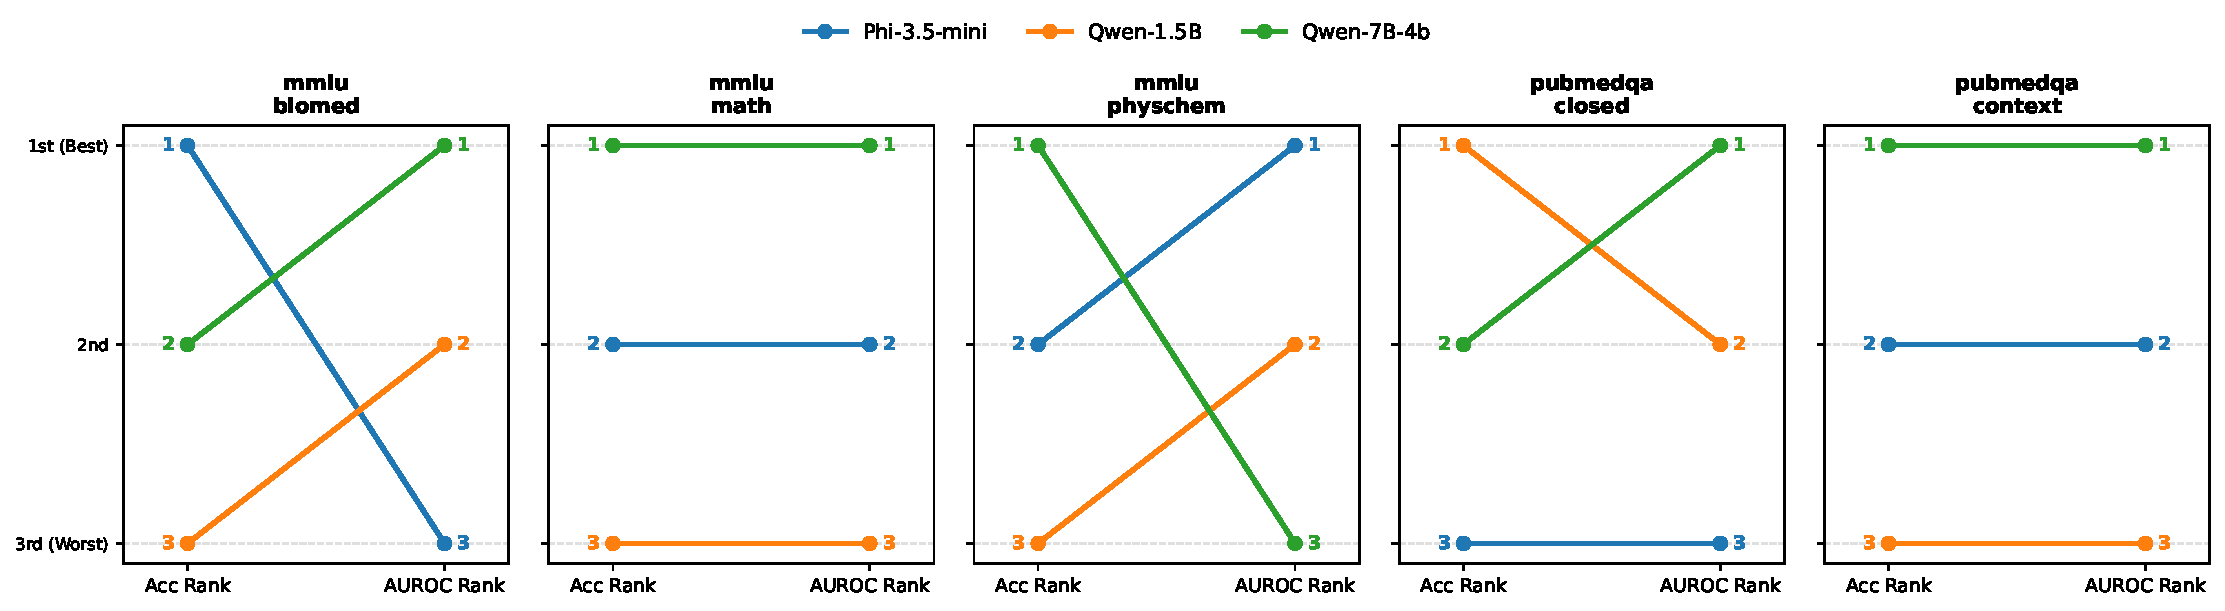
\includegraphics[width=\textwidth]{figures/fig_rank_inversion_slopegraph.pdf}
\caption{Rank inversion slopegraph: model ranking by Raw Accuracy (left) vs Confidence Discrimination ($\text{AUROC}_{\text{conf}}$, right) across slices. Rank flips are descriptive; most MMLU accuracy differences are not statistically significant (Table~\ref{tab:paired}), and AUROC confidence intervals overlap for the model pairs whose ranks flip (\texttt{results.csv}).}
\label{fig:slopegraph}
\end{figure*}

\begin{table*}[!t]
\centering
\caption{RQ2: Effect of providing abstract context on PubMedQA (context minus closed-book). $p$-values are Holm-adjusted McNemar tests.}
\label{tab:taskmode}
\small
\fitwidth{\textwidth}{% RQ2 context minus closed-book (PubMedQA)
\resizebox{\columnwidth}{!}{%
\begin{tabular}{lllll}
\toprule
Model & $\Delta\text{Acc}$ [95\% CI] & $\Delta\text{ECE}$ [95\% CI] & $\Delta\text{Brier}$ [95\% CI] & McNemar $p$ (Holm) \\
\midrule
phi-3.5-mini-instruct & 0.336 [0.286, 0.390] & -0.305 [-0.359, -0.250] & -0.613 [-0.715, -0.516] & $<$0.001 \\
qwen2.5-1.5b-instruct & 0.108 [0.072, 0.146] & -0.016 [-0.056, 0.020] & -0.123 [-0.176, -0.068] & $<$0.001 \\
qwen2.5-7b-instruct-4bit & 0.310 [0.256, 0.364] & -0.275 [-0.331, -0.220] & -0.571 [-0.671, -0.475] & $<$0.001 \\
\bottomrule
\end{tabular}%
}
}
\end{table*}

\begin{table*}[!t]
\centering
\caption{POST HOC exploratory evaluation: balanced accuracy and macro-F1 on PubMedQA under closed-book and context-grounded modes.}
\label{tab:balanced_posthoc}
\small
\fitwidth{\textwidth}{% POST HOC exploratory: balanced accuracy and macro-F1 on PubMedQA
\resizebox{\textwidth}{!}{%
\begin{tabular}{lllll}
\toprule
Model & Slice & Acc & Balanced acc [95\% CI] & Macro-F1 [95\% CI] \\
\midrule
phi-3.5-mini-instruct & pubmedqa\_closed & 0.324 & 0.350 [0.298, 0.399] & 0.267 [0.232, 0.301] \\
phi-3.5-mini-instruct & pubmedqa\_context & 0.660 & 0.600 [0.546, 0.655] & 0.583 [0.541, 0.623] \\
qwen2.5-1.5b-instruct & pubmedqa\_closed & 0.552 & 0.372 [0.342, 0.401] & 0.352 [0.315, 0.391] \\
qwen2.5-1.5b-instruct & pubmedqa\_context & 0.660 & 0.450 [0.425, 0.475] & 0.429 [0.398, 0.458] \\
qwen2.5-7b-instruct-4bit & pubmedqa\_closed & 0.418 & 0.342 [0.296, 0.387] & 0.291 [0.256, 0.326] \\
qwen2.5-7b-instruct-4bit & pubmedqa\_context & 0.728 & 0.587 [0.541, 0.636] & 0.592 [0.546, 0.637] \\
\bottomrule
\end{tabular}%
}
}
\end{table*}

\begin{figure*}[!t]
\centering
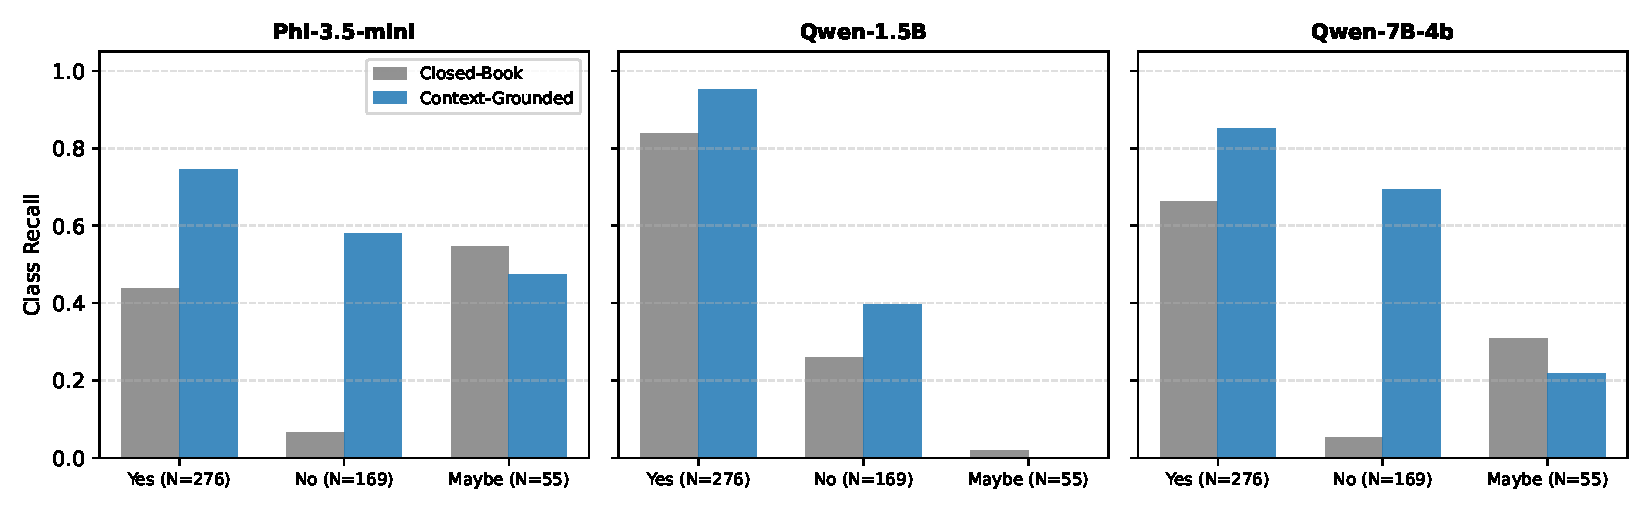
\includegraphics[width=\textwidth]{figures/fig_pubmedqa_class_recall_shift.pdf}
\caption{Per-class recall on PubMedQA under closed-book vs context-grounded evaluation.}
\label{fig:class_recall}
\end{figure*}

\subsection{RQ2: Evidence Grounding Shifts and Strong Yes-Bias}\label{sec:rq2}
Table~\ref{tab:taskmode} and Figure~\ref{fig:class_recall} summarize the impact of providing published abstracts on PubMedQA. For \textsf{Phi-3.5-mini} and \textsf{Qwen2.5-7B}, context substantially improves performance: accuracy increases by $+33.6$ points and $+31.0$ points respectively (paired McNemar $p < 0.001$), accompanied by substantial reductions in calibration error: $\Delta\text{ECE} = -0.305$ and $-0.275$ (from \texttt{task\_mode\_delta.csv}), followed by $\Delta\text{Brier} = -0.613$ and $-0.571$, noting that Brier score inherently conflates accuracy and calibration. Per-class recall and McNemar gain/loss counts for all three models are listed in Table~\ref{tab:pubmedqa_detail}.

In closed-book mode, \textsf{Qwen2.5-1.5B} achieves an apparent accuracy of $55.2\%$, exceeding both larger models ($32.4\%$ and $41.8\%$; Table~\ref{tab:main}). However, analysis of the classification confusion matrix demonstrates that this is an artifact of majority-class prediction:
\begin{itemize}
    \item The 500 PubMedQA evaluation items comprise 55.2\% `yes' ($N=276$), 33.8\% `no' ($N=169$), and 11.0\% `maybe' ($N=55$).
    \item In closed-book mode, \textsf{Qwen2.5-1.5B} predicted `yes' for 391 of 500 questions ($78.2\%$). Its raw accuracy of 55.2\% matches the 55.2\% majority class share purely by coincidence; its recall on `no' was 26.0\% and on `maybe' was 1.8\% (Figure~\ref{fig:class_recall}).
    \item This affirmative bias persists directly across both evaluation regimes: when provided with full abstract context, \textsf{Qwen2.5-1.5B}'s prediction rate for `yes' further intensifies to 82.6\% (413 of 500 predictions), achieving 95.3\% recall on `yes' ($263/276$) but failing completely on `maybe' with 0.0\% recall ($0/55$) and only 39.6\% recall on `no' ($67/169$).
    \item To formally verify this effect, Table~\ref{tab:balanced_posthoc} reports balanced accuracy and macro-F1 (POST HOC and EXPLORATORY; not in the fixed protocol (\protocolfile, version 1.0, seed 42)). In closed-book mode, \textsf{Qwen-1.5B} achieves a balanced accuracy of only 0.372 [0.342, 0.401] and macro-F1 of 0.352 [0.315, 0.391]. Even with context, balanced accuracy reaches only 0.450 and macro-F1 0.429 due to total collapse on the `maybe' class.
\end{itemize}

The closed-book collapse is not specific to \textsf{Qwen2.5-1.5B}, and it does not always point toward `yes' (descriptive; counts taken from the raw per-item outputs). \textsf{Phi-3.5-mini} predicted `maybe' for 276 of 500 closed-book questions ($55.2\%$), `yes' for 205 ($41.0\%$), and `no' for only 19 ($3.8\%$), although `maybe' is the gold label for just $11.0\%$ of the items. Its closed-book recall is therefore $54.5\%$ on `maybe' ($30/55$) but only $43.8\%$ on `yes' ($121/276$) and $6.5\%$ on `no' ($11/169$; Table~\ref{tab:pubmedqa_detail}), which yields a raw accuracy of $32.4\%$ and a balanced accuracy of $0.350$, barely above the $1/3$ chance level (Table~\ref{tab:balanced_posthoc}). Thus the low closed-book accuracy of \textsf{Phi-3.5-mini} reflects a `maybe' bias rather than a lack of calibrated uncertainty about the claim. When the abstract is provided, its `maybe' predictions fall from 276 to 140 and its recall on `no' rises from $6.5\%$ to $58.0\%$ (Figure~\ref{fig:class_recall}). \textsf{Qwen2.5-7B} is yes-leaning in closed-book mode (308 `yes', 172 `maybe', and 20 `no' predictions). Across all three models, `no' is the most under-predicted class without context: 19, 93, and 20 `no' predictions for \textsf{Phi-3.5-mini}, \textsf{Qwen2.5-1.5B}, and \textsf{Qwen2.5-7B} respectively, against 169 gold `no' items. Closed-book collapse can therefore go to a hedge class as well as to the majority class, so class-balanced metrics are needed in both cases.

\begin{table*}[!t]
\centering
\caption{RQ3: Permutation consistency vs correctness per cell; stubborn-error mean confidence ranges from 0.813 to 1.000 across cells.}
\label{tab:consistency}
\small
\fitwidth{\textwidth}{% RQ3 consistency vs correctness
\resizebox{\textwidth}{!}{%
\begin{tabular}{llcccc}
\toprule
Model & Slice & $N$ & $\text{AUROC}_{\text{cons}}$ [95\% CI] & Consistently Wrong & Share of Errors \\
\midrule
phi-3.5-mini-instruct & mmlu\_biomed & 150 & 0.679 [0.590, 0.773] & 0.113 & 0.500 \\
phi-3.5-mini-instruct & mmlu\_math & 150 & 0.657 [0.570, 0.739] & 0.113 & 0.215 \\
phi-3.5-mini-instruct & mmlu\_physchem & 150 & 0.745 [0.669, 0.823] & 0.120 & 0.281 \\
phi-3.5-mini-instruct & pubmedqa\_closed & 500 & 0.432 [0.383, 0.482] & 0.438 & 0.648 \\
phi-3.5-mini-instruct & pubmedqa\_context & 500 & 0.558 [0.513, 0.601] & 0.224 & 0.659 \\
qwen2.5-1.5b-instruct & mmlu\_biomed & 150 & 0.688 [0.603, 0.774] & 0.133 & 0.435 \\
qwen2.5-1.5b-instruct & mmlu\_math & 150 & 0.671 [0.588, 0.760] & 0.073 & 0.118 \\
qwen2.5-1.5b-instruct & mmlu\_physchem & 150 & 0.632 [0.552, 0.706] & 0.233 & 0.427 \\
qwen2.5-1.5b-instruct & pubmedqa\_closed & 500 & 0.561 [0.524, 0.597] & 0.316 & 0.705 \\
qwen2.5-1.5b-instruct & pubmedqa\_context & 500 & 0.556 [0.525, 0.589] & 0.276 & 0.812 \\
qwen2.5-7b-instruct-4bit & mmlu\_biomed & 150 & 0.679 [0.600, 0.760] & 0.147 & 0.550 \\
qwen2.5-7b-instruct-4bit & mmlu\_math & 150 & 0.731 [0.652, 0.805] & 0.113 & 0.262 \\
qwen2.5-7b-instruct-4bit & mmlu\_physchem & 150 & 0.761 [0.682, 0.839] & 0.087 & 0.245 \\
qwen2.5-7b-instruct-4bit & pubmedqa\_closed & 500 & 0.661 [0.619, 0.701] & 0.290 & 0.498 \\
qwen2.5-7b-instruct-4bit & pubmedqa\_context & 500 & 0.632 [0.589, 0.672] & 0.174 & 0.640 \\
\bottomrule
\end{tabular}%
}
}
\end{table*}

\begin{figure*}[!t]
\centering
\begin{subfigure}{0.48\textwidth}
    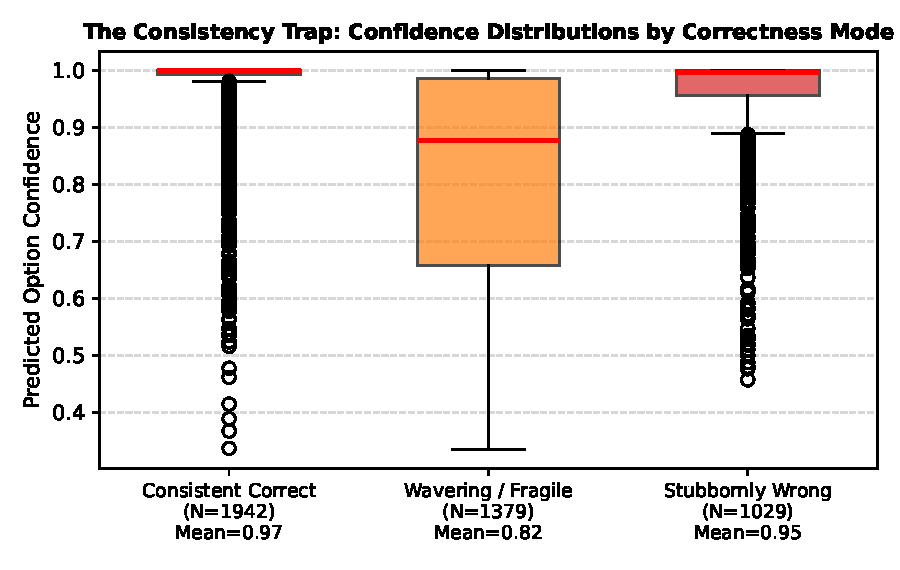
\includegraphics[width=\textwidth]{figures/fig_stubborn_confidence_distribution.pdf}
    \caption{Confidence distribution across correctness modes.}
    \label{fig:stubborn_box}
\end{subfigure}
\hfill
\begin{subfigure}{0.48\textwidth}
    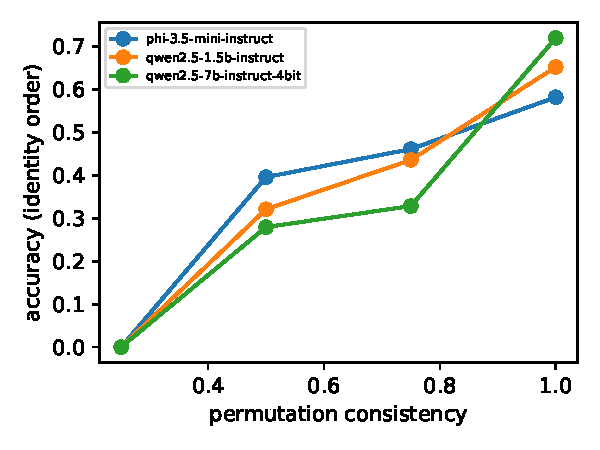
\includegraphics[width=\textwidth]{figures/fig_accuracy_by_consistency.pdf}
    \caption{Observed accuracy vs consistency level.}
    \label{fig:acc_by_cons}
\end{subfigure}
\caption{The consistency trap. (a) Boxplot of predicted confidence distributions across Consistent Correct ($N=1{,}942$), Wavering ($N=1{,}379$, items whose prediction changed across orders, whether correct or not), and Stubbornly Wrong ($N=1{,}029$) groups across all 4,350 evaluations ($N = 1{,}942 / 1{,}379 / 1{,}029$, total 4,350). (b) Accuracy by consistency level across slices ($N=5$ items at $\text{Cons}=0.25$, $N=548$ at $0.50$, $N=826$ at $0.75$, $N=2{,}971$ at $1.00$). Pooling across slices masks cells where the consistency-accuracy relationship is reversed: for \textsf{Phi-3.5-mini} in closed-book PubMedQA, only 82 of 301 fully consistent items are correct (27.2\%; Table~\ref{tab:stubborn_detail}).}
\label{fig:consistency_depth}
\end{figure*}

\subsection{RQ3: The Consistency Trap and Stubborn Errors}\label{sec:rq3}
Table~\ref{tab:consistency} reports consistency metrics across all cells. As shown in Figure~\ref{fig:acc_by_cons}, accuracy generally increases with consistency level. However, across all 15 cells, we identify \textbf{1,029 stubborn wrong instances} where models repeat the identical incorrect choice across all four option permutations ($\text{Cons} = 1.0, \text{Acc} = 0.0$).

Stubborn errors account for \textbf{54.6\% of all errors} ($1{,}029 / 1{,}885$; per-cell counts in Table~\ref{tab:stubborn_detail}). Per cell, the stubborn share of errors ranges from 11.8\% (\textsf{Qwen-1.5B} math) to 81.2\% (\textsf{Qwen-1.5B} \textsf{pubmedqa\_context}; Table~\ref{tab:consistency}). As shown in Figure~\ref{fig:stubborn_box}, stubborn errors exhibit high mean confidence: overall mean confidence is $0.949$, with cell means ranging from $0.813$ to $1.000$ (reaching $1.000$ for \textsf{Phi-3.5} on biomed). As a hypothesis suggested by qualitative inspection of three examples (rather than a measured taxonomy of all 1,029 errors), stubborn errors may arise from two candidate mechanisms: (a) \textit{parametric misconceptions}, where an incorrect choice is selected across all option orders, or (b) \textit{deficit-driven defaults}, where an ungrounded model predicts an epistemic hedge (such as `maybe') or majority option in the absence of context.

Table~\ref{tab:consistency} also reports $\text{AUROC}_{\text{cons}}$. Notably, on closed-book PubMedQA for \textsf{Phi-3.5-mini}, $\text{AUROC}_{\text{cons}} = 0.432$ (95\% CI $[0.383, 0.482]$), falling below 0.5. In this cell, consistency is inversely related to accuracy: consistent predictions are more likely to be wrong than wavering ones due to 219 stubborn errors. By construction, consistency-based checks cannot identify stubborn errors because the model produces identical predictions across permutations.

\section{In-Depth Analysis}
\subsection{Failure Case Examination}
Inspection of stubborn failure cases suggests two candidate failure mechanisms:
\begin{enumerate}
    \item \textbf{Parametric Misconceptions (Entrenched Priors):} Models may exhibit invariant selection of an incorrect option regardless of presentation order:
    \begin{itemize}
        \item \textbf{Item \texttt{mmlu-anatomy-25}:} \textit{``Which of the following substances is found in greater quantity in exhaled air?''} Options: [Carbon dioxide, Carbon monoxide, Nitrogen, Oxygen]. Gold: Nitrogen. All three models consistently select Carbon dioxide across all 4 permutations with confidences $1.0000$ for \textsf{Phi-3.5}, $0.8871$ for \textsf{Qwen-1.5B}, and $1.0000$ for \textsf{Qwen-7B} ($\text{Cons} = 1.0$ for all three).
        \item \textbf{Item \texttt{mmlu-astronomy-42}:} \textit{``Why is Saturn almost as big as Jupiter despite its smaller mass?''} Gold: \textit{``Jupiter's greater mass compresses it more thus increasing its density.''} Both \textsf{Phi-3.5} and \textsf{Qwen-1.5B} consistently select the distractor citing hydrogen and helium proportions with $\text{Cons} = 1.0$ (confidences $1.0000$ and $0.8458$), while \textsf{Qwen-7B} selected the same distractor on the canonical order with confidence $1.0000$ but wavered across permutations ($\text{Cons} = 0.5$).
    \end{itemize}
    \item \textbf{Deficit-Driven Defaults (Uncertainty Collapse):} In the absence of evidence, models may default to an epistemic hedge or default class:
    \begin{itemize}
        \item \textbf{Item \texttt{pubmedqa-10966337}:} \textit{``A short stay or 23-hour ward in a general and academic children's hospital: are they effective?''} Gold: `yes'. In closed-book mode, \textsf{Phi-3.5} predicts `maybe' across all permutations ($\hat{c} = 1.0000, \text{Cons} = 1.0$). When provided with abstract context, its prediction shifts to the correct answer `yes' ($\hat{c} = 1.0000, \text{Cons} = 1.0$).
    \end{itemize}
\end{enumerate}

\subsection{Display Position Bias Audit}
\label{sec:pos_bias}
We evaluated option display frequencies across permuted presentations (descriptive analysis). For 4-choice MMLU items where uniform selection corresponds to 25.0\%, models display observable display position preferences. \textsf{Phi-3.5-mini} selected option position `B' 34.0\% in math and 30.2\% in physchem (compared to 17.7\% and 22.2\% for `A'). \textsf{Qwen2.5-1.5B} selected position `B' 38.2\% in math, while selecting position `D' only 11.8\% of the time. In contrast, \textsf{Qwen2.5-7B-Instruct-4bit} displayed more uniform selection rates across all three MMLU slices from \texttt{position\_bias.csv}: on math, options A, B, C, and D were selected 24.3\%, 27.7\%, 25.3\%, and 22.7\% of the time (maximum deviation from uniform: 2.7 points at `B'); on physical sciences, 26.7\%, 26.7\%, 22.8\%, and 23.8\% (maximum deviation: 2.2 points at `C'); and on biomedicine, 25.0\%, 26.2\%, 23.8\%, and 25.0\% (maximum deviation: 1.2 points at `B' and `C'). Across all MMLU slices, the maximum position-bias deviations from 25.0\% were 2.7 points for \textsf{Qwen2.5-7B}, 9.0 points for \textsf{Phi-3.5-mini} (math `B' at 34.0\%), and 13.2 points for \textsf{Qwen2.5-1.5B} (math `B' at 38.2\%).

\subsection{Confidence Discrimination vs Consistency}
Comparing $\text{AUROC}_{\text{conf}}$ and $\text{AUROC}_{\text{cons}}$ across all 15 cells (Tables~\ref{tab:main} and~\ref{tab:consistency}), confidence discrimination exceeds consistency discrimination in 12 of 15 cells. Across all cells, the mean difference is $+0.042$; over the 12 cells where confidence exceeds consistency, the mean difference is $+0.063$.

\subsection{Permutation Ensembling (Exploratory)}
\label{sec:ensembling}
Averaging predicted probabilities across all four option permutations ($\text{Acc}_{\text{ens}}$; exploratory analysis without paired hypothesis testing) produces accuracy differences ($\Delta = \text{Acc}_{\text{ens}} - \text{Acc}$) spanning $-0.027$ to $+0.067$ across all 15 cells:
\begin{itemize}
    \item \textbf{Biomedical MMLU:} \textsf{Phi-3.5-mini}: $0.773 \to 0.773$ ($\Delta = 0.000$); \textsf{Qwen2.5-1.5B}: $0.693 \to 0.667$ ($\Delta = -0.027$); \textsf{Qwen2.5-7B}: $0.733 \to 0.740$ ($\Delta = +0.007$).
    \item \textbf{Mathematics MMLU:} \textsf{Phi-3.5-mini}: $0.473 \to 0.480$ ($\Delta = +0.007$); \textsf{Qwen2.5-1.5B}: $0.380 \to 0.447$ ($\Delta = +0.067$); \textsf{Qwen2.5-7B}: $0.567 \to 0.580$ ($\Delta = +0.013$).
    \item \textbf{Physical Sciences MMLU:} \textsf{Phi-3.5-mini}: $0.573 \to 0.593$ ($\Delta = +0.020$); \textsf{Qwen2.5-1.5B}: $0.453 \to 0.500$ ($\Delta = +0.047$); \textsf{Qwen2.5-7B}: $0.647 \to 0.673$ ($\Delta = +0.027$).
    \item \textbf{PubMedQA Closed-Book:} \textsf{Phi-3.5-mini}: $0.324 \to 0.308$ ($\Delta = -0.016$); \textsf{Qwen2.5-1.5B}: $0.552 \to 0.564$ ($\Delta = +0.012$); \textsf{Qwen2.5-7B}: $0.418 \to 0.452$ ($\Delta = +0.034$).
    \item \textbf{PubMedQA Context-Grounded:} \textsf{Phi-3.5-mini}: $0.660 \to 0.638$ ($\Delta = -0.022$); \textsf{Qwen2.5-1.5B}: $0.660 \to 0.660$ ($\Delta = 0.000$); \textsf{Qwen2.5-7B}: $0.728 \to 0.732$ ($\Delta = +0.004$).
\end{itemize}
Ensembling improved accuracy in 10 cells, produced no change in 2 cells, and decreased accuracy in 3 cells.

\section{Discussion: What a Leaderboard Should Show}
\paragraph{Leaderboard Reporting Recommendations.}
Our findings demonstrate that single-number accuracy rankings do not capture multi-dimensional model reliability. We recommend that scientific benchmarks report a multi-dimensional scorecard: (1) Raw Accuracy; (2) Probability Calibration (Brier score / ECE); (3) Selective Accuracy (at 80\% coverage); and (4) Permutation Consistency. While permutation averaging improved accuracy in 10 of 15 cells (3 decreased, 2 unchanged; Section~\ref{sec:ensembling}), it cannot correct errors that are identical across all four orders. When model probability mass collapses decisively onto a single incorrect option irrespective of order, order-invariance cannot serve as a safeguard of truth.

\paragraph{Vulnerabilities of Closed-Book Scientific QA}
Closed-book evaluation on imbalanced datasets carries severe risks of rewarding models that collapse onto majority classes. Evaluating without context controls or class-balanced metrics can produce misleading benchmarks.

\paragraph{Scale and Positional Stability.}
Among the MMLU slices, \textsf{Qwen2.5-7B} is the most positionally stable model: its maximum deviation from uniform option selection is 2.7 points on math, compared to 9.0 points for \textsf{Phi-3.5-mini} and 13.2 points for \textsf{Qwen2.5-1.5B}. This suggests that scale may help suppress superficial positional heuristics, though we cannot disentangle scale from architecture and training data.

\paragraph{Practitioner Deployment Checklist.}
Based on our empirical findings, we offer a three-point protocol for evaluating and deploying language models in scientific domains:
\begin{enumerate}
    \item \textbf{Autonomous and Safety-Critical Pipelines:} Prioritize selective accuracy at high coverage ($\text{SelAcc}_{0.8}$) and confidence discrimination ($\text{AUROC}_{\text{conf}}$) over raw accuracy. When models cluster within sampling noise (e.g., $p \in [0.35, 0.98]$ on biomedicine), selective accuracy may reduce operational risk by abstaining on uncertain queries.
    \item \textbf{Literature and RAG Retrieval-QA:} Mandate balanced accuracy and macro-F1 alongside raw accuracy. On imbalanced clinical benchmarks like PubMedQA, models can achieve ostensibly competitive accuracy (55.2\%; Table~\ref{tab:balanced_posthoc}) via a strong yes-bias while suffering large recall failure on minority classes.
    \item \textbf{Robustness Auditing:} Pair permutation consistency with evidence grounding controls rather than treating order invariance as a standalone proxy for correctness. Consistency checks cannot detect stubborn errors (identical across all four option orders), which constitute 54.6\% of all errors.
\end{enumerate}

\section{Limitations and Threats to Validity}
Several limitations qualify our findings:
\begin{enumerate}
    \item \textbf{Model Scale and Sample Size:} We evaluated three small-to-medium models ($1.5\mathrm{B}$ to $7\mathrm{B}$). With $N=3$ models per slice, rank correlations have wide confidence intervals and paired differences on some slices are non-significant.
    \item \textbf{Quantization Confound:} \textsf{Qwen2.5-7B} was evaluated in 4-bit NF4 precision, whereas \textsf{Qwen2.5-1.5B} and \textsf{Phi-3.5-mini} were evaluated in full 16-bit precision.
    \item \textbf{Prompt Template Sensitivity:} Evaluations used a single chat prompt template per dataset. Results may vary under different prompt formulations.
    \item \textbf{Item-Level Resampling:} Bootstrap confidence intervals resample test items, reflecting item-level variance rather than stochasticity in model weights.
    \item \textbf{Benchmark Contamination:} Pre-training data contamination was not audited.
    \item \textbf{Dataset Artifacts:} MMLU items may contain minor label noise, and PubMedQA has an imbalanced class distribution (11\% `maybe' class).
    \item \textbf{Task Scope:} This study evaluates multiple-choice QA correctness, calibration, selective prediction, and permutation consistency; it does not evaluate open-ended generation, temporal validity, or step-by-step reasoning proofs.
\end{enumerate}

\section{Conclusion}
This study evaluated whether factuality metrics rank small open LLMs concordantly on scientific question answering. Across 17,400 forward passes, we found that Brier score and selective accuracy track raw accuracy, while calibration error and confidence discrimination diverge. Evidence context rescues accuracy on PubMedQA, whereas ungrounded evaluation can reward a strong yes-bias. Furthermore, permutation consistency does not detect stubbornly held errors, which constitute over half of all error instances. Scientific benchmark reporting should adopt multi-dimensional scorecards separating accuracy, calibration, and presentation stability.

\bibliographystyle{ACM-Reference-Format}
\bibliography{refs}

\appendix
\section{Evaluation Prompt Templates}
All models were evaluated using zero-shot multiple-choice letter scoring (next-token probabilities over the option letters) under standardized prompt templates. All prompts are sent as a user message in each model's official chat template. Candidate options are displayed in permuted order (display position $j$ displays option $\pi(j)$). For PubMedQA context-grounded mode, the abstract text is truncated at 6,000 characters.

\subsection{MMLU Science Subsets (Chat Style)}
\begin{quote}
\small\ttfamily\raggedright
The following is a multiple-choice question about \{subject\}. Respond with only the letter of the correct answer.\\[0.6\baselineskip]
Question: \{question\}\\
A. ...\\
B. ...\\
C. ...\\
D. ...\\
Answer:
\end{quote}

\subsection{PubMedQA Closed-Book (Chat Style)}
\begin{quote}
\small\ttfamily\raggedright
Answer the following biomedical research question.\\[0.6\baselineskip]
Question: \{question\}\\
A. yes B. no C. maybe\\
Respond with only the letter of your answer.
\end{quote}

\subsection{PubMedQA Context-Grounded (Chat Style)}
\begin{quote}
\small\ttfamily\raggedright
Read the abstract and answer the research question based on it.\\[0.6\baselineskip]
Abstract:\\
\{abstract\}\\[0.6\baselineskip]
Question: \{question\}\\
options\\
Respond with only the letter of your answer.
\end{quote}

\subsection{Baseline Validation Harness Prompt}
The harness-style prompt mimicking EleutherAI's \textsf{lm-evaluation-harness}:
\begin{quote}
\small\ttfamily\raggedright
The following are multiple choice questions (with answers) about \{subject\}.\\[0.6\baselineskip]
\{question\}\\
\{options\}\\
Answer:
\end{quote}
was used \textbf{only} for baseline validation; it was not used for comparative model evaluations.

\section{Computing Environment and Hyperparameters}
Evaluation runs across the 3 models totaled 17,400 forward passes (3 models $\times$ 1,450 item-slice evaluations $\times$ 4 permutations). All inference was executed under the recorded execution environment:
\begin{itemize}
    \item \textbf{Hardware:} NVIDIA Tesla T4 GPU.
    \item \textbf{Software Stack:} Python 3.13.16, PyTorch 2.14.1+cu130, and HuggingFace Transformers 4.45.2.
    \item \textbf{Model Quantization and Precision:}
    \begin{itemize}
        \item \textsf{Qwen2.5-1.5B-Instruct}: Evaluated in 16-bit floating point (\texttt{float16}).
        \item \textsf{Phi-3.5-mini-instruct}: Evaluated in 16-bit floating point (\texttt{float16}).
        \item \textsf{Qwen2.5-7B-Instruct-4bit}: Evaluated in 4-bit NormalFloat (NF4) via \texttt{bitsandbytes} using library defaults (\texttt{load\_in\_4bit=True}, \texttt{bnb\_4bit\_compute\_dtype=torch.float16}, \texttt{bnb\_4bit\_quant\_type="nf4"}; \texttt{bnb\_4bit\_use\_double\_quant} left at its default (\texttt{False}), no double quantization).
    \end{itemize}
    \item \textbf{Inference Settings:} Batch size 8, deterministic option permutations $K = 4$, random seed 42, protocol version 1.0.
\end{itemize}

\section{Additional Statistical Tables}
Table~\ref{tab:stubborn_detail} gives the per-cell breakdown of consistency modes and stubborn errors discussed in Section~\ref{sec:rq3}, and Table~\ref{tab:pubmedqa_detail} gives the per-class recall shifts and McNemar counts discussed in Section~\ref{sec:rq2}.

\begin{table*}[!t]
\centering
\caption{Detailed breakdown of stubborn confident errors and consistency modes across all 15 cells.}
\label{tab:stubborn_detail}
\small
\setlength{\tabcolsep}{3.5pt}
\fitwidth{\textwidth}{% Detailed breakdown of stubborn confident errors and consistency modes across all 15 cells
\resizebox{\textwidth}{!}{%
\begin{tabular}{llrrrrrrrrrr}
\toprule
Model & Slice & $N$ & Consistent Correct $N$ & Consistent Correct Pct & Wavering $N$ & Wavering Pct & Stubborn Wrong $N$ & Stubborn Wrong Pct & Mean Conf Correct & Mean Conf Wavering & Mean Conf Stubborn Wrong \\
\midrule
phi-3.5-mini-instruct & mmlu\_biomed & 150 & 99 & 66.0 & 34 & 22.7 & 17 & 11.3 & 0.981 & 0.952 & 1.000 \\
phi-3.5-mini-instruct & mmlu\_math & 150 & 31 & 20.7 & 102 & 68.0 & 17 & 11.3 & 0.942 & 0.871 & 0.916 \\
phi-3.5-mini-instruct & mmlu\_physchem & 150 & 64 & 42.7 & 68 & 45.3 & 18 & 12.0 & 0.967 & 0.883 & 0.972 \\
phi-3.5-mini-instruct & pubmedqa\_closed & 500 & 82 & 16.4 & 199 & 39.8 & 219 & 43.8 & 0.913 & 0.853 & 0.976 \\
phi-3.5-mini-instruct & pubmedqa\_context & 500 & 257 & 51.4 & 131 & 26.2 & 112 & 22.4 & 0.967 & 0.873 & 0.980 \\
qwen2.5-1.5b-instruct & mmlu\_biomed & 150 & 80 & 53.3 & 50 & 33.3 & 20 & 13.3 & 0.919 & 0.757 & 0.920 \\
qwen2.5-1.5b-instruct & mmlu\_math & 150 & 20 & 13.3 & 119 & 79.3 & 11 & 7.3 & 0.751 & 0.654 & 0.813 \\
qwen2.5-1.5b-instruct & mmlu\_physchem & 150 & 46 & 30.7 & 69 & 46.0 & 35 & 23.3 & 0.918 & 0.776 & 0.853 \\
qwen2.5-1.5b-instruct & pubmedqa\_closed & 500 & 228 & 45.6 & 114 & 22.8 & 158 & 31.6 & 0.871 & 0.670 & 0.901 \\
qwen2.5-1.5b-instruct & pubmedqa\_context & 500 & 305 & 61.0 & 57 & 11.4 & 138 & 27.6 & 0.944 & 0.726 & 0.960 \\
qwen2.5-7b-instruct-4bit & mmlu\_biomed & 150 & 99 & 66.0 & 29 & 19.3 & 22 & 14.7 & 0.983 & 0.886 & 0.970 \\
qwen2.5-7b-instruct-4bit & mmlu\_math & 150 & 62 & 41.3 & 71 & 47.3 & 17 & 11.3 & 0.940 & 0.844 & 0.907 \\
qwen2.5-7b-instruct-4bit & mmlu\_physchem & 150 & 70 & 46.7 & 67 & 44.7 & 13 & 8.7 & 0.955 & 0.869 & 0.942 \\
qwen2.5-7b-instruct-4bit & pubmedqa\_closed & 500 & 171 & 34.2 & 184 & 36.8 & 145 & 29.0 & 0.940 & 0.854 & 0.966 \\
qwen2.5-7b-instruct-4bit & pubmedqa\_context & 500 & 328 & 65.6 & 85 & 17.0 & 87 & 17.4 & 0.978 & 0.840 & 0.960 \\
\bottomrule
\end{tabular}%
}
}
\end{table*}

\begin{table*}[!t]
\centering
\caption{PubMedQA deep dive: class recall shifts and McNemar test breakdown.}
\label{tab:pubmedqa_detail}
\small
\setlength{\tabcolsep}{3.5pt}
\fitwidth{\textwidth}{% PubMedQA deep dive: class recall shifts and McNemar test breakdown
\resizebox{\textwidth}{!}{%
\begin{tabular}{lrrrrrrrrrrrr}
\toprule
Model & Closed Acc & Closed Rec Yes & Closed Rec No & Closed Rec Maybe & Context Acc & Context Rec Yes & Context Rec No & Context Rec Maybe & $\Delta$Acc & Gain ($b$) & Loss ($c$) & McNemar $p$ (Holm) \\
\midrule
phi-3.5-mini-instruct & 0.324 & 0.438 & 0.065 & 0.545 & 0.660 & 0.746 & 0.580 & 0.473 & 0.336 & 198 & 30 & $<$0.001 \\
qwen2.5-1.5b-instruct & 0.552 & 0.837 & 0.260 & 0.018 & 0.660 & 0.953 & 0.396 & 0.000 & 0.108 & 77 & 23 & $<$0.001 \\
qwen2.5-7b-instruct-4bit & 0.418 & 0.663 & 0.053 & 0.309 & 0.728 & 0.851 & 0.692 & 0.218 & 0.310 & 186 & 31 & $<$0.001 \\
\bottomrule
\end{tabular}%
}
}
\end{table*}

\end{document}